\documentclass[]{article}
\usepackage[latin1]{inputenc}
\usepackage[T1]{fontenc}
\usepackage[english]{babel}
\usepackage{amsmath}
\usepackage{amssymb,amsfonts,textcomp}
\usepackage{color}
\usepackage{array}
\usepackage{supertabular}
\usepackage{hhline}
\usepackage{hyperref}
\hypersetup{pdftex, colorlinks=true, linkcolor=blue, citecolor=blue, filecolor=blue, urlcolor=blue, pdftitle=PUML TOME OF USE, pdfauthor=Theora Rice, pdfsubject=, pdfkeywords=}
\usepackage[pdftex]{graphicx}
\usepackage{verbatim}

\begin{document}
\title{
Project: UML\linebreak 
\textbf{Tome of Use}}
\author{Team Pummel}
\maketitle

\newpage
{\centering\selectlanguage{english}\bfseries\color{black}
TABLE OF CONTENTS
\par}
{\selectlanguage{english}\bfseries\color{black}
Section\ \ Page}
\setcounter{tocdepth}{9}
\renewcommand\contentsname{}
\tableofcontents

\newpage
\section{Introduction}
{\selectlanguage{english}\color{black}
Welcome to Project: UML PUML, the UML Diagramming editor designed in the 2011-2013 Software Engineering class at the University of Idaho. This program has been designed to try and accurately create and replicate certain UML Diagrams for use by future computer science students. All work put into this program has been completed in nine months by eight computer science majors, using the Qt Designer framework. In the following pages reside the instructions on how to use PUML to edit and create class, use case, and state chart diagrams. Good luck in your diagramming pursuits. - Team Pummel
\linebreak
Supported Platforms : \newline
Windows \newline
Linux (Refer to Known Bugs Section)\newline

NOTE: A hint box is provided in PUML. This is located under the 'Help' tab Click on 'Hints and Tips' and a box will appear giving the user some general editing information that may not be obvious. 
}

\section{UML Diagram Types}
{\selectlanguage{english}\color{black}
One can create a use case, class, and state chart diagram using the PUML program. Each of these different types have limitations in what objects and connections are allowed. In future versions of this product more diagramming types will be added, with similar object restrictions and connection rules. 
}
\section{Installing the Program}
{\selectlanguage{english}\color{black}
For Windows, an installer is provided. Click and download pummel.exe, and then follow the steps to download it to your personal computer. 
}
\subsection{Layout}
{\selectlanguage{english}\color{black}
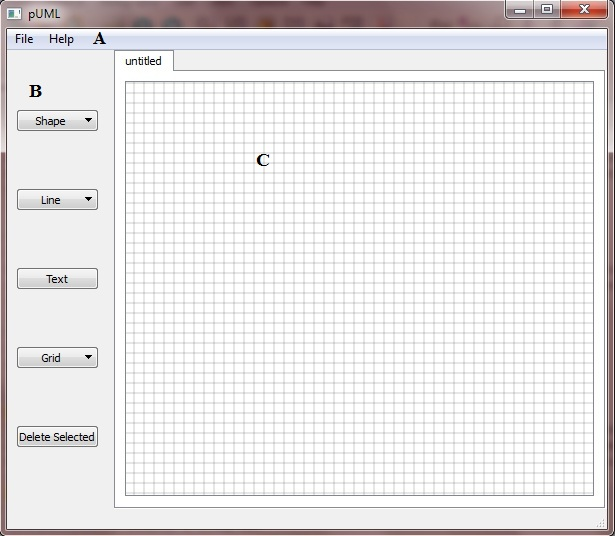
\includegraphics[scale = .60]{Layout}

The layout of the program is depicted above. (Slight graphic variations have been observed in different operating systems.) 
A. The top bar of the window is used for file operations and overall program functionality. Help is also found here.
B. This is called the Toolbar, and is there for the user to reference how to edit the icons and drawing area.
C. This is the drawing area where UML Diagrams are created. 
}

\section{General Editing}
\subsection{To Create a Diagram}
{\selectlanguage{english}\color{black}
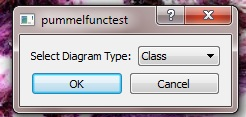
\includegraphics[scale = .70]{StartMenu}

In order to create a diagram, one must open the PUML Program. A pop up will ask what type of diagram you wish to create. Select a type from the drop down menu and click 'Ok', or 'Cancel' if you wish to exit the program and start another time.
}
\subsection{Tabs}
\subsubsection{To Open a New Tab}
{\selectlanguage{english}\color{black}
In order to open a new tab -and a new type of diagram-, click 'File' and select 'New Tab' from the drop down menu. The same dialogue from the beginning of the program will pop up, allowing the user to choose a diagram type for the new tab. 
}
\subsubsection{To Close a New Tab}
{\selectlanguage{english}\color{black}
In order to close an open tab, one must be operating in the tab one wishes to close. Then click 'File', 'Close Tab.' A window will appear asking if the user wishes to save any progress made on the diagram within the tab. Once the user has clicked 'Save', 'Don't Save', or 'Cancel' the tab will close.
}
\subsection{Turning the Grid On/Off}
{\selectlanguage{english}\color{black}
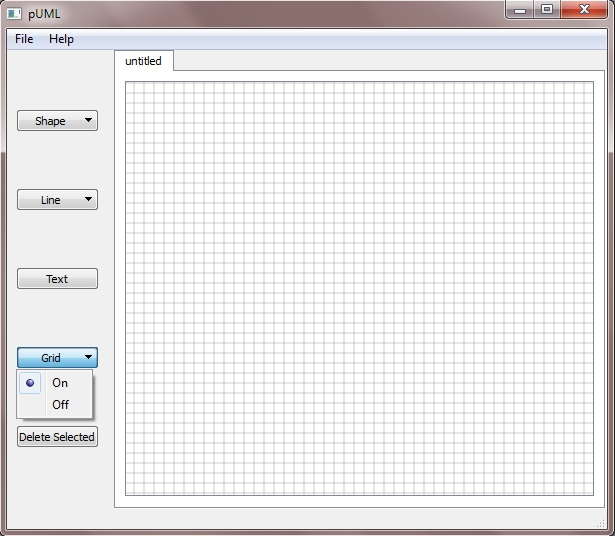
\includegraphics[scale = .50]{Gridonoff}

In order to provide more structure for UML Diagram creation, PUML includes an optional grid. To view the grid, click the 'Grid On/Off' button on the toolbar. Select 'On' from the drop down menu, and the grid will appear on the drawing area. To turn the grid off, select the same button and select 'Off.'
}
\subsection{Icon Management}
\subsubsection{To Create an Icon}
{\selectlanguage{english}\color{black}
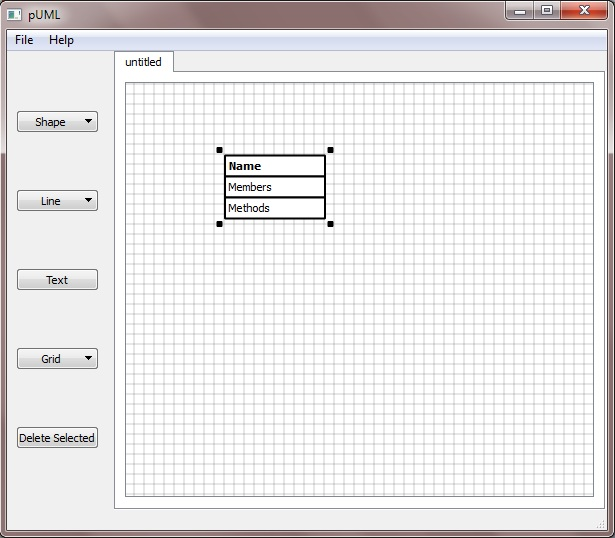
\includegraphics[scale = .50]{CreateIcon}

To create an icon to use in a diagram, click the  'Shape' button on the left side of the screen. Select what the shape to be created from the drop down list, and then click on the drawing area to create the icon. 
}
\subsubsection{To Delete an Icon}
{\selectlanguage{english}\color{black}
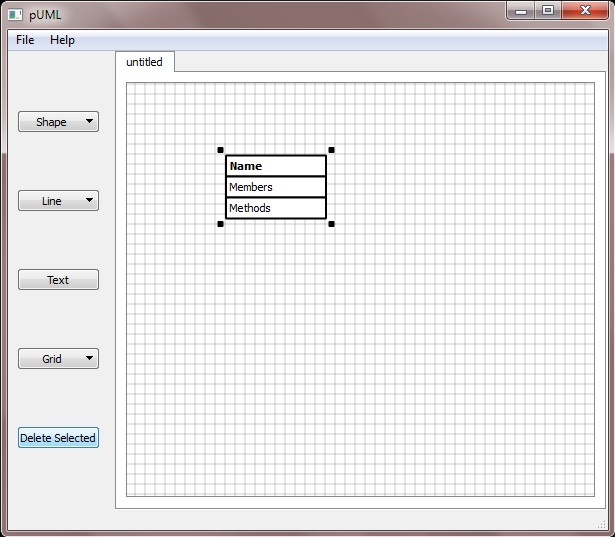
\includegraphics[scale = .50]{DeletingIcon}

To delete an icon, select the icon with the cursor. Then click the bottom button on the toolbar that states 'Delete Object.'
}
\subsubsection{To Resize an Icon}
{\selectlanguage{english}\color{black}
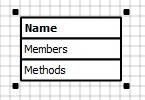
\includegraphics[scale = .70]{Resizing}

To resize an icon, select the individual icon with the cursor. Four small boxes will appear at the corners of the icon. To resize, drag one of these boxes outside or into the icon depending on whether the user wants to make the icon larger or smaller. Release the cursor, and the icon will be resized. 
}
\subsection{Line Management}
\subsubsection{To Create a Line}
{\selectlanguage{english}\color{black}
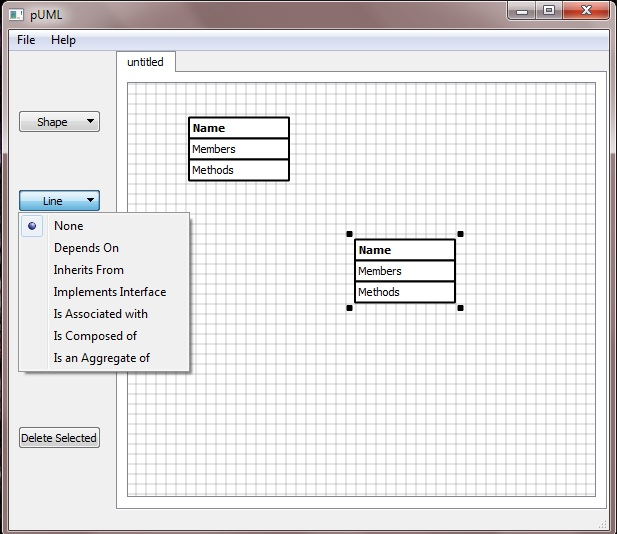
\includegraphics[scale = .50]{ChoosingLine}

In order to create a line, click the line button on the toolbar and select a line type from the drop down list. Then, select one of the two icons you wish to connect in the drawing area, and drag the cursor to the other icon. A line will be created based on the selection. 

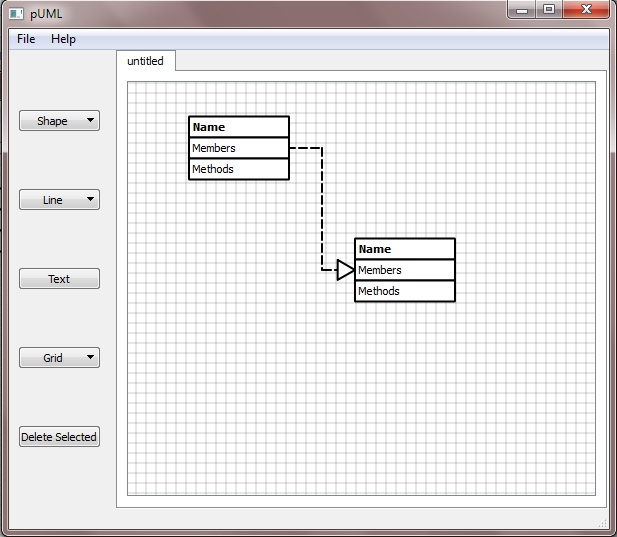
\includegraphics[scale = .45]{CreatedLine}
}
\subsubsection{To Delete a Line}
{\selectlanguage{english}\color{black}
In order to delete a line, one of the icons it is attached to must be deleted. This is a documented bug. 
}
\section{Saving Your Document}
\subsection{Saving a Diagram}
{\selectlanguage{english}\color{black}
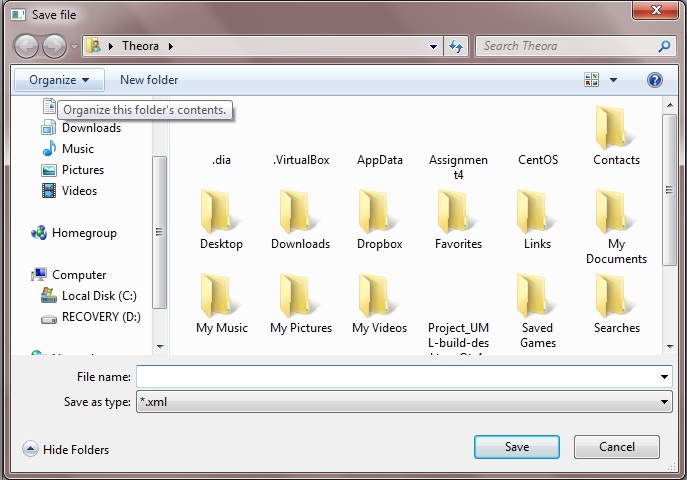
\includegraphics[scale = .50]{SaveAsFile}

To preserve a diagram, click on the 'File' tab in the upper left hand side of the screen. From the drop down menu, select 'Save Diagram.' A dialogue box will pop up with a map of the current directory and a text box to contain the name. Enter the name desired and navigate to the correct directory for file storage. The diagram will be saved as an XML file within the system. 
}
\subsection{Opening a Saved Diagram}
{\selectlanguage{english}\color{black}
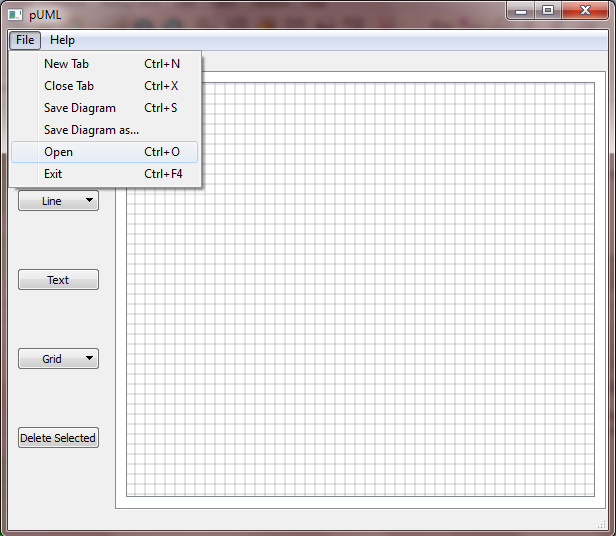
\includegraphics[scale = .50]{Open}

To open a diagram, click on the 'File' tab and select 'Open' from the dropdown list. A dialogue box will appear with a map of the current directory. Navigate to the folder which the sought file resides in, and select the file. Click 'Open' and it will be ready for editing. 
}
\section{List of Known Bugs}
{\selectlanguage{english}\color{black} 
\begin{list}{-}{ }
\item LINUX SPECIFIC: Save feature does not function correctly. This is a documented error in the Qt framework.
\item Cannot select or delete lines individually
\end{list}
}
\section{More Information}
{\selectlanguage{english}\color{black}
For more information, refer to one of the following documents:
\begin{list}{-}{ }
\item ``System and Software Design Description (SSDD): Incorporating Architectural Views and Detailed Design Criteria for Project: UML''
\item ``System and Software Requirements Specification (SSRS) for PUML: Project UML''
\item ``Test Plan for Project UML (PUML): A UML Diagramming Tool for the 2012 CS 384 Class Version 1.0''
\end{list}
}
\end{document}
